\documentclass{jsarticle}
\usepackage[margin = .7in]{geometry}
\usepackage[dvipdfmx]{graphicx}
\usepackage{listings}
\usepackage{amsmath}
\usepackage{bm}
\lstset{%
  language={python},
  basicstyle={\small},%
  identifierstyle={\small},%
  commentstyle={\small\itshape},%
  keywordstyle={\small\bfseries},%
  ndkeywordstyle={\small},%
  stringstyle={\small\ttfamily},
  frame={tb},
  breaklines=true,
  columns=[l]{fullflexible},%
  numbers=left,%
  xrightmargin=0zw,%
  xleftmargin=3zw,%
  numberstyle={\scriptsize},%
  stepnumber=1,
  numbersep=1zw,%
  lineskip=-0.5ex%
}



\begin{document}
\title{給付型奨学金の効果検証}
\author{Kei Ikegami}
\maketitle

\section{事実}
    \begin{itemize}
    	\item Jassoの予約採用募集時期は5,6月に1種2種、10,11月に2種のみ。在学採用は毎年春。ただし詳しい時期や回数は高校に一任されている。
    \end{itemize}
    
\section{モデルの設定}
	\subsection{モデル1:池上/12/22}
	ナイーブなモデルを設定する。
	\par
	全国の高校生は3年生の5、6月に、以下のプロセスをバックワードに意思決定する。
	\begin{enumerate}
		\item 進学するか否か
		\item 受験する学校(職場)のセットは何か
	\end{enumerate}
	受験する学校のセットは以下のように決定される。$A$を国公立4年生大学、$B$を私立4年生大学、$C$を専門学校の集合とする。$A,B,C$の各学校は奨学金ありと奨学金なしで2パターンずつ存在する。受験生は$A$の中から効用を最大化する選択肢を1つ選び、$B,C$については効用の高い順にランク付けする。$A$から選んだものも含めてすべての選択肢についてのランキングを作成した後、受験生が住んでいる都道府県での受験校平均だけ上から取り出したものを受験校のセットとする(ただし正の値のもののみを含むようにする)。
	\par
	生徒$i$が学校$n$の奨学金なしパターンを選択する効用を$u_n^i$とすると、
	\begin{align*}
		u_n^i = (I_n - H^i - T_n) r_n^i
	\end{align*}
	ただし、$I_n$は学校$n$を卒業した人の平均生涯賃金、$H^i$は$i$さんが住んでいる都道府県の高卒者平均生涯賃金、$T_n$は学校$n$の学費の割引現在価値、$r_n^i$は$i$さんが学校$n$に受かる確率である。\par
	奨学金ありパターンを選択する効用を${u_n^i}^{*}$とすると、
	\begin{align*}
		{u_n^i}^{*} = (u_n^i + S_n^i - P^i - C - \infty * {\bf 1}(X_i \in Q)) r_n^i d^i
	\end{align*}
	ただし、$S_n^i$は$i$さんが学校$n$に進学した際にもらえる奨学金の合計金額の割引現在価値、$P^i$は$i$さんが返済する金額の割引現在価値、$C$は奨学金に申し込むコスト、$X_i$は$i$さんのdemographicで$Q$が奨学金をもらえないdemographicの集合である。また、$d_n^i$は$i$さんの奨学金採用確率である。
	\par
	上で述べた通り、学生は各学校について上の二つの効用を比べ、効用最大化問題を解いている。
	\par
	進学せずに就職するやつの数を、「受験校のセットが空集合の受験生の数」+「(各学校に対する合格率で当落を判定し、すべて不合格になった受験生の数)×$\ w$」(ただし$w$は全落ちしたやつが浪人せずに就職する確率)で推定する。上の効用をパラメトライズして、この高卒就職組の数を高校別or県別に出してMLEをすればいい?
	
	\subsection{モデル1改良:池上12/24,5}
	\par
	モデル1をもう少しspecificにする。
	\begin{itemize}
		\item 意思決定に自宅通学か下宿かの分岐を入れ込んじゃう
		\item 大学のcharacteristicsとして「関関同立」のような世間一般に受け入れられている格付けをを追加
		\item specficationとして各大学の受験生獲得シェアの学費弾力性のようなものを推定するようにパラメトライズする。→この文脈だと国公立に絞った方が嬉しいかも?(一つしか選べないので)
	\end{itemize}
	\par
	疑問としては次のものがある。
	\begin{itemize}
		\item 流動性制約をこのモデルで扱えているか?
		\item そもそも奨学金もらっている人が少ないし、torbitとかのほうがいいのかな?
	\end{itemize}
	\par
	以下で具体的に書く。
	$s = 0$で自宅通学、$s = 1$で下宿を表す。$a = 0$で奨学金なし、$a = 1$で奨学金受給を表す。$i$さんが学校$n$に$s, a$の状態で通うことの効用を以下のように書く。
	\begin{align*}
	u_{i,n,s,a} = &\left\{ y_n{\bf \beta_i} + \alpha_i \left( T_n - {\bf 1(a = 1)} A_i\right) + \gamma_i H_n + \delta_i {\bf 1(s = 1)} S_n + \eta_i R_i - {\bf 1(a = 1)}\left( {\bf 1(X_i \in Q_n)} * \infty \right) \right\}\\
	 & * r_n(X_i) * \left\{ p(X_i) {\bf 1(a = 1)}\right\}
	\end{align*}
	ここで、$y_n$は学校$n$の、就職という選択肢と比べられる特徴量(例えば生涯賃金)。$T_n$は学校$n$の学費の現在価値、$A_i$は$i$さんが貰える奨学金の現在価値である。$H_n$は学校$n$の「格」を表す指標で、「東大・京大」「早稲田・慶應」などの大学間のランク付けが社旗通念として一般に受け入れられていることから取り入れる価値があると判断した。これは順序付きのカテゴリー変数でもいいし、格ごとのダミー変数でもいい。$S_n$は学校$n$に下宿で通う場合の家賃である。学校周辺のワンルームの平均家賃をデータとして用いる(通っている間の割引現在価値を入れる)。$R_i$は$i$さんが返済する奨学金の金額の割引現在価値である。現在でも返済うる金額には差異が存在しているようなのでその変動を利用する。$X_i$はiさんのdemographicで、$Q$が奨学金の対象である個人のdemographic空間ないの部分集合である。$r_n(X_i)$は$i$さんの学校$n$に対する合格率で、$X_i$の関数で書く。$p(X_i)$は$i$さんの奨学金採用率で、これも$X_i$の関数で書く。式中の${\bf 1}$はindicator functionである。ただし、上式での各パラメータは個人に依存した形にしているので、実際に計算するときはBLPみたいにmean utilityとheteroな部分に分解して計算することになるので注意(めんどくさいしとりあえずhomogeneticなモデルでやるのがいいかも)。
	\par
	先のモデルと同様に、$i$さんの県内での平均受験校数を$N_i$として、国公立から最大の効用をもたらす学校を一つ、私立と専門から効用の大きい順に$N_i -1$個選び、$N_i$この受験校bundleを作る。それと、就職する効用である$u_{i, 0}$とを比べて、就職するシェアを離散選択モデルの文脈で計算する。そのシェアに、bundleに全落ちする学生のうちから何割かを浪人せずに就職する人達として、そのシェアに追加し、全体としての高卒就職率を算出する。
	\par
	浪人せずに就職する割合をbeta分布などからシミュレーションして、Farmanian and Salanie (2004)に基づいてlikelihood functionを作成すし、MLEを求める。(それかそれもパラメータとしてただのMLEでやる)
	
	\subsection{モデル2:池上12/28}
	意思決定の過程は以下のとおり。主体は高校3年生とその世帯とする。
	\par
	まず、高校3年生は以下の2パターンに分類される。
	\begin{enumerate}
		\item 奨学金なしで通うことのできる学校が存在する
		\item 奨学金なしではどの学校にも通うことができない
	\end{enumerate}
	ここで、「通うことのできる学校が存在する」とは実現可能性集合に高校以降の学校が少なくとも一つ含まれている状態を指す。学校に関する情報は完全であることを仮定し、存在するすべての学校に対して世帯ごとに通悪可能かいなかが判断されている状態を想定する。下宿も自宅通学もどちらの可能性も考慮して実現可能か否かは判断されることとする。
	\par
	パターン1の学生はそれぞれ「通うことのできる学校リスト($A$と呼称)」を入手する。「奨学金がもらえる時に通うことのできる学校リスト($B$と呼称)」も同時に作成され、その際に以下の3パターンに分割できる。
	\begin{description}
		\item[$1-a$] $A$の中で効用最大化を達成する選択肢が$B$の中で効用最大化を達成する選択肢と一致する。
		\item[$1-b$] $A$と$B$とで効用最大化を達成する選択肢が異なる。
		\item[$1-c$] 奨学金制度をよく知らず、Aしか見ることができない。
	\end{description}
	簡単のために$1-a$は奨学金に申し込まないとする。$1-b$は$B$における最大の効用が受験しないという選択肢の効用を上回った時のみ奨学金への申し込みを行う。奨学金の採択確率は$X_i$を$i$さんのdemographicとして$q(X_i)$でかけるとする。$1-c$は奨学金を申し込まない。
	\par
	また2のパターンの学生は以下の2パターンに分類できる。
	\begin{description}
		\item[$2-a$] 奨学金を知っている。それによって「奨学金があったら通えるリスト($C$と呼称)」が与えられる。
		\item[$2-b$] 奨学金を知らない。
	\end{description}
	この時$2-a$はCにおける最大効用が受験しないという選択肢の効用を上回った時のみ勉強を始め、奨学金に申し込む。$2-b$は受験することはできない。
	\par
	上で、各学生は自分のリストから最大の効用を与える学校と受験しないという選択肢を比べて「勉強を始める」という意思決定を行い、パターンによっては「奨学金に申し込む」という意思決定も行う。次に、彼らは受験をするか否かという意思決定を行うために、自分の受験校のbundleを決定する。このbundleの決定は受験というくじの価値を決めるものである。bundleの決定は単純に、「仮にその学校に受かったとして、受験しないで就職するよりはいいことがありそうだ」と思えないものはbundleに入れない問いうルールに従うとする。$i$さんのbundleにはいる学校の個数は「$i$さんの在住県の学生が受験する学校の平均数」と「受験しないという選択肢よりも大きな効用をもたらす、$i$さんのリスト内にある学校の数」の小さい方と等しいとする。
	\par
	学生たちは次に「受験するかしないか」の意思決定を行う。bundleの決定によりくじの価値が決定したのでこの意思決定を考えることができる。$i$さんのbundleを$B_i$とする。$B_i$には$1,2, \dots, m_i$だけ学校が入っており、それぞれに$r_{i,1}, r_{i,2}, \dots, r_{i,m_i}$が$i$さんの合格率として紐付いており、それぞれの合格した際の効用を$u_{i, 1}, u_{i, 2}, \dots, u_{i, m_{i}}$と表記することとする。
	\par
	bundleないの学校は数字が小さいほど$i$さんにとっての効用が大きいとして、より効用が大きい学校に受かればそれ以下の学校には進学しないとして、すべての学校に落ちた時の効用を$b_{i, 0}$とすると、$B_i$の持つ期待効用は以下のように書ける。
	\begin{align*}
		u_i^* &= r_{i, 1}b_{i, 1} + (1-r_{i, 1})r_{i, 2} b_{i, 2} + \dots + \Pi_{j = 1}^{m_i - 1} (1 - r_{i, j}) r_{i, m_{i}} b_{i, m_{i}} + \Pi_{j = 1}^{m_{i}} (1 - r_{i, j}) b_{i, 0} 
	\end{align*}
	今、$u_i$を$i$さんが就職する際の効用として、誤差項にType 1 extreme value distributionを仮定すれば離散選択モデルとして高卒就職を意図的に選択する人のシェアを出すことができる。
	\par
	最後に今まで扱ってきた効用を以下のようにパラメトライズする。$i$さんが学校$j$に奨学金なしで進学し、そこで学位をとることの効用を$u_{i, j}$とし、$i$さんが学校$j$に奨学金付きで進学しそこで学位をとることの効用を$\dot{u_{i, j}}$とする。この時以下のようである。
	\begin{align*}
		&u_{i, j} = \alpha_i \sum_{n = 1}^{L_j} \left\{ h^n (y_i^n - t_j - w_i^n) \right\} + \alpha_i \sum_{n = L_j + 1}^{\infty} \left\{ h^n (y_i^n + z_j^n - w_i^n) \right\} + \beta_i d_j + \delta_i C_{i, j} \\
		&\dot{u_{i, j}} = \alpha_i \sum_{n = 1}^{L_j} \left\{ h^n (y_i^n - t_j - w_i^n + s_i) \right\} + \alpha_i \sum_{n = L_j + 1}^{\infty} \left\{ h^n (y_i^n + z_j^n - w_i^n - r_i^n) \right\} + \beta_i d_j + \delta_i C_{i, j} 
	\end{align*}
	ここで、
	\begin{description}
		\item[$y_i^n$] 世帯$i$の$n$年後の世帯収入
		\item[$w_i^n$] $i$さんが高卒で就職した際の$n$年後の収入
		\item[$r_i^n$] $i$さんが大学進学して$n$年後に返済する奨学金の額
		\item[$z_j^n$] $j$校を卒業した学生が$n$年後に稼いでいる年収
		\item[$d_j$] $j$校の「格」を示すカテゴリー変数(ダミーにしても良い)
		\item[$C_{i, j}$] $i$さんが$j$校に「合格」し、「学位を所得」するまでに必要な勉強コスト(必要な時間でバイトした時の収入増加分の割引現在価値)
		\item[$L_j$] $j$校で学位をとるまでに必要な年限
		\item[$h$] 割引率
	\end{description}
	である。
	
	\subsection{モデル2改良:池上12/29}
	浪人するという意思決定をモデルに組み込む。まず$i$さんの浪人可能年数を$Y_i$とする。$Y_i$は
	\begin{align*}
		Y_i = \# e\  \text{s.t.}\  \exists j\ \text{s.t.}\ b_{i, j}^{e} \geq u_{i, 0}^{e}
	\end{align*}
	で定義される。すなわち、「$i$さんが$e$浪して合格した時の効用が$e$回受験に失敗した時に就職した時の効用よりも大きくなる学校$j$が少なくとも一つ存在している年数」である。
	\par
	2.3節とほぼ同じ記号を使って、以下のように「$i$さんが$j$校に$e$浪して合格した時の効用」を新しく定義する。
	\begin{align}
		&u_{i, j}^e = \alpha_i \sum_{n = 1}^{e} \left\{ h^n(-f_j - w_i^n) \right\} \alpha_i \sum_{n = 1+e}^{L_j+e} \left\{ h^n (- t_j - w_i^n) \right\} + \alpha_i \sum_{n = L_j +e+ 1}^{\infty} \left\{ h^n (z_j^{n-e} - w_i^n) \right\} \nonumber\\
		&\quad \quad+ \beta_i d_j + \delta_i C_j + \eta_i g_j + \gamma e \\[10pt]
		&\dot{u_{i, j}}^e = \alpha_i \sum_{n = 1}^{e} \left\{ h^n(-f_j - w_i^n) \right\} \alpha_i \sum_{n = 1+e}^{L_j+e} \left\{ h^n (- t_j - w_i^n + s_i) \right\} + \alpha_i \sum_{n = L_j +e+ 1}^{\infty} \left\{ h^n (z_j^{n-e} - w_i^n - r_i) \right\} \nonumber\\
		&\quad \quad+ \beta_i d_j + \delta_i C_j + \eta_i g_j + \gamma e 
	\end{align}
	ただし
	\begin{description}
		\item[$f_j$] $j$校に受かるための浪人費用1年分
		\item[$C_j$] $j$校の偏差値
		\item[$g_j$] $j$校を卒業した場合の配偶者の期待所得
	\end{description}
	である。
	\par
	上の効用を用いて、$i$さんのbundleの持つ価値が以下のように書ける。
	\begin{align}
		u_i^* = \sum_{e = 0}^{Y_i} (1 - \epsilon)^e u_i^e + \epsilon \sum_{e = 0}^{Y_i - 1} (1 - \epsilon)^e u_{i, 0}^e + (1 - \epsilon)^{Y_i} u_{i, 0}^{Y_i}
	\end{align}
	ただし、
	\begin{align}
		&u_i^e = r_{i, 1}^e b_{i, 1}^e + \dots + \Pi_{j = 1}^{m_i^e} (1 - r_{i, j}) r_{i, m_{i}^{e}}^e b_{i, m_{i}^{e}}^e\\[8pt]
		&u_{i, 0}^e = \alpha_i \sum_{n = 0}^{\infty} (h^n w_i^{n-e} )
	\end{align}
	また、$b_{i, j}^e = \max(u_{i, j}^e, \dot{u_{i, j}}^e)$、$r_{i, j}^e$は$i$さんが$e$浪で$j$校に受かる確率、$m_i^e$が$i$さんの$e$浪目のbundleには入っている学校である。$\epsilon$はすべての志望校に不合格となった場合に次年度浪人することが可能なのにもかかわらず就職することを選んでしまう確率である。
	$(3)$の構成は以下の図を参考にする。($e = 3$とかで試すとわかる)
	\begin{center}
	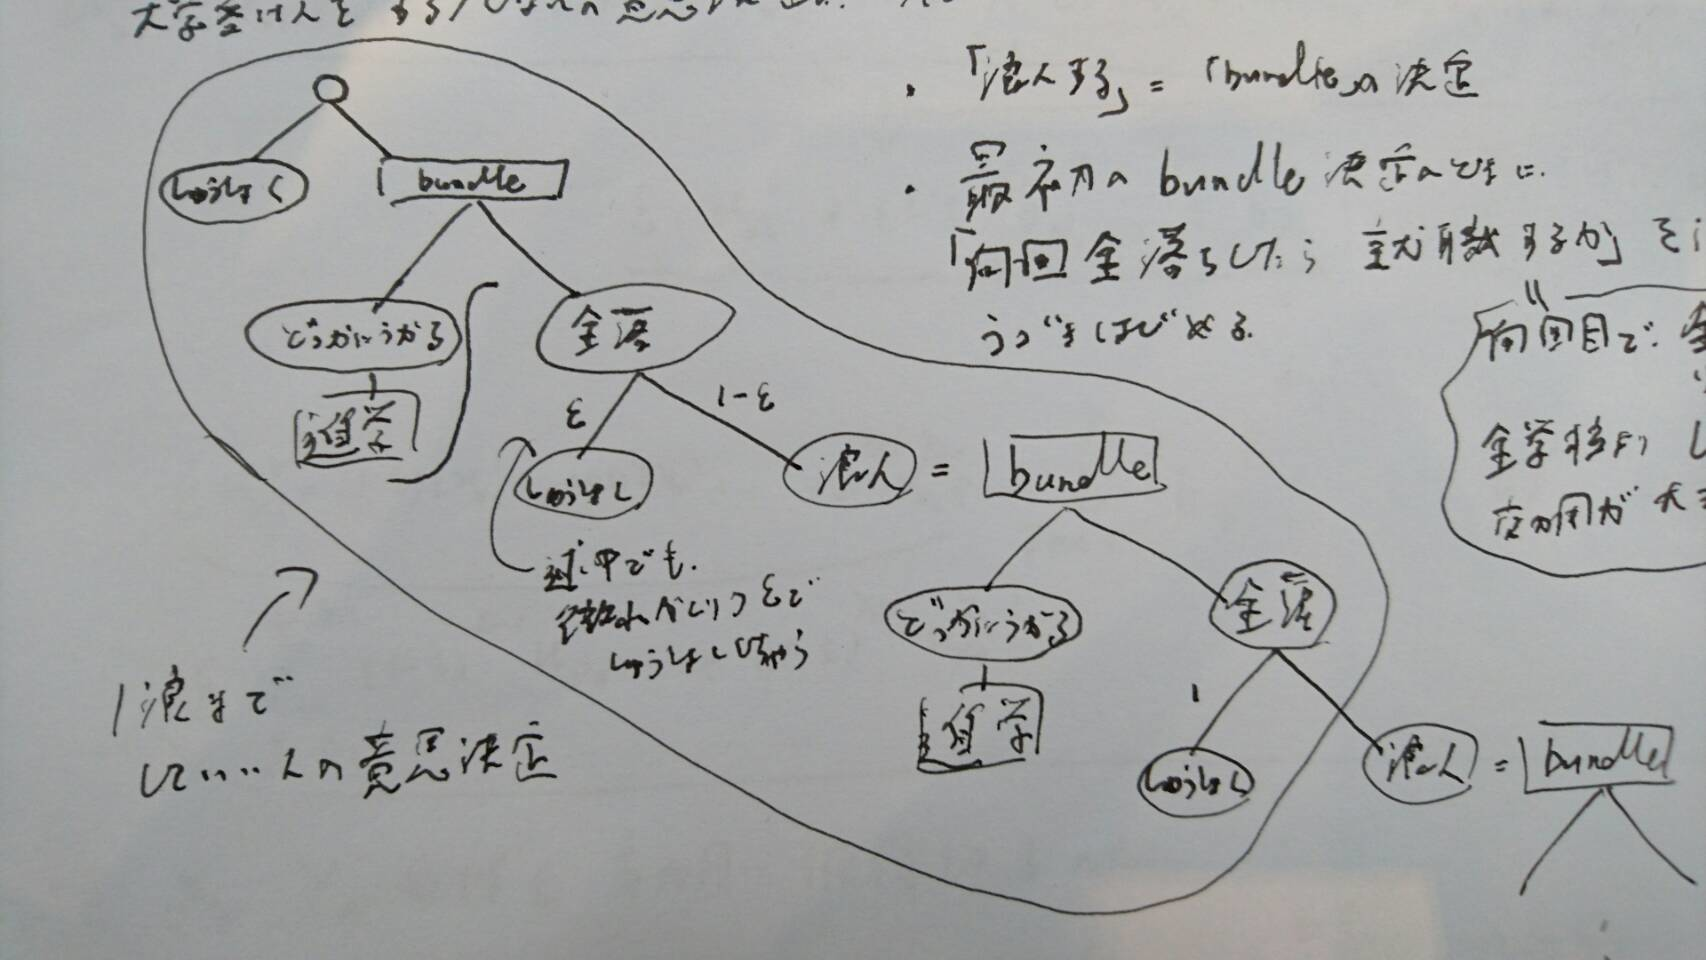
\includegraphics[width = 12cm]{fig1.png}
	\end{center}
	
	\section{分析}
	\subsection{分析1:RD(徳田)}
	
	\subsection{分析1改良:RD(池上)}
	
	\subsection{分析2:ヘテロな離散選択(池上)}
	$n_1$を1種奨学金申請者数、$n_2$を2種奨学金申請者数、$n_3$を1種2種併用奨学金申請者数、$n_4$を奨学金に申請せずに進学を希望する人数、$n_5$を進学を希望しない人数、とする。$n_1, n_2, n_3$はJassoのデータからわかる。$n_4$は各大学の倍率と合格者数のデータから合計志望者数を計算し$n_1,n_2,n_3$の合計をそこから引くことで計算する。$n_5$はデータがあるので簡単にわかる。
	\par
	使えるデータは「いずれかの奨学金に申請した家計に関する諸変数」、「いずれかの奨学金に申請した家計がどの奨学金を選択したかの離散データ」、「各奨学金がいくらを支給しいくらの返済を求めるか」である。「奨学金に申し込まなかった家計に関する変数」は知りようがないことに注意する。これらのデータから上の5つの選択肢に関する離散選択モデルの文脈で、ヘテロな効用関数を推定することを考える。
	\par
	$j = 1,2,3,4,5$であり、$T$年分のデータが得られているとする。$p_{jt}$を選択肢$j$の$t$年における割引現在価値とする。ここで、割引現在価値は「払う総額の割引現在価値からもらう総額の割引現在価値を引いいたもの」と「大卒資格の有無による生涯所得の変化」、「大学に通う間労働しない分の機会費用」から計算する。また各選択肢がこの$p_{jt}で完全に特徴付けられているとする。$$y_i$を家計$i$の世帯収入、$Z_i$を家計iについての諸変数をまとめたベクトル、$\xi_{jt}$を家計に共通の観測できないショック、$\epsilon_{ijt}$を家計レベルの観測できないショックとする。
	\par
	この時家計$i$の$j$に対する$t$年の効用($u_{ijt}$)を以下のように書く。ただし、$a_i$は家計$i$の変数に依存したパラメータであり、$a_i = a + \Pi_aZ_i + \Sigma_a\upsilon_{i}$でかけるものとする。この時$\upsilon_{i}$は標準正規分布からの乱数として、$a$と$\Pi_a$と$\Sigma_a$が推定したいパラメータとなる。
	\begin{align}
		u_{ijt} &= a_i (y_i - p_{jt}) + Z_i^{'}\beta + \xi_{jt} + \epsilon_{ijt} \nonumber \\
		&= a_i y_i + Z_i^{'}\beta + (-a p_{jt} + \xi_{jt}) + (-\Pi_a Z_i - \Sigma_a \upsilon_i )p_{jt} + \epsilon_{ijt} \nonumber \\
		&= a_i y_i + Z_i^{'}\beta + \delta_{jt} + \mu_{ijt} + \epsilon_{ijt}
	\end{align}
	ここで$\epsilon_{ijt}$が第1種極値分布に従っているとすると、
	\begin{align}
		q_{ijt} = \frac{\exp{\delta_{jt} + \mu_{ijt}}}{\sum_k \exp{\delta_{kt} + \mu_{ikt}}} \nonumber
	\end{align}
	として、
	\begin{align}
		q_{ijt}^{*} = \int_{\upsilon_i} q_{ijt} \mathrm{d} P_{\upsilon_i}(\upsilon_i)
	\end{align}
	が家計$i$の$j$に対する$t$年の選択確率である。これは$a, \xi_{jt}, \Pi_a, \Sigma_a$を未知の値とする関数としてかけている($\xi_{jt}$は$j$ごとに別々のパラメータとすればいい?)。この選択確率を利用して奨学金申請者のデータから尤度関数を作成し、パラメータの最尤推定量を求める。これを初期値として以下のBLPっぽい推定を行う(BLPは推定の精度がクソらしいのでそれっぽい初期値を持ってきてあげると良くなりそうだなと思ってる)。
	\par
	各選択肢のシェアは以下のように計算できる。
	\begin{align}
		s_{jt} = \int_{Z} \int_{\upsilon_i} q_{ijt}\ \mathrm{d}Z\ \mathrm{d}\upsilon_i
	\end{align}
	ここで以下のループを回す。
	\begin{enumerate}
		\item パラメータをgivenとして(最初は上で求めたMLE)シェアを(8)式に従って計算する。
		\item 計算したシェアに基づいて$\delta$に関する以下の縮小写像を使い$\delta$を更新する。更新式は$\delta_t^{h+1} = \delta_t^h + ({\rm log}(S_t) - {\rm log}(s_t))$であり、$S_t$は実際の各選択肢のシェアで$s_t$がシミュレーションしたシェアである。それぞれの変数が選択肢ごとの値を含むベクトルとなっていることに注意。
		\item 更新した$\delta$を$p_{jt}$と定数項に回帰し、$a$と$\xi_{jt}$を更新する。
		\item 更新した$a$と$\xi$に基づいて、$\omega = \delta - (-a p_{jt} + \xi_{jt})$を計算し、$\omega^{'}(E(\omega^{'} \omega))^{-1} \omega$を最小化するような$\Pi_a, \Sigma_a$をnumericalに求める
		\item 更新されたすべてのパラメータを使ってループの1に戻る。
	\end{enumerate}
	これが収束するまで回してパラメータを推定する。
	
	
\end{document}
































